\documentclass[letterpaper]{article}
\usepackage[spanish]{babel}
\usepackage[utf8]{inputenc}
\usepackage{graphicx}
\usepackage{amsmath}

\title{Bitácora del proyecto}
\author{Acuña Yeomans Eduardo}
\date{}

\begin{document}

\maketitle

\section{Sobre esta bitácora}
Este escrito es una bitácora de desarrollo en donde le daré seguimiento a un proyecto de desarrollo de software.

El texto está escrito de manera informal pero técnica y está escrito para que sea leído por el profesor asesor del proyecto Adrián Vazquez Osorio y por los integrantes del equipo de trabajo Daniel Contreras Mejía y Francisco Manuel Valle Ruiz. La bitácora se va construyendo de manera temporal y contendrá descripciones sobre las entregas de trabajos asociadas al proyecto, los fallos o errores con los que nos encontramos en el transcurso del desarrollo y observaciones tanto del profesor asesor como de los integrantes del equipo sobre el trabajo realizado.

Mi nombre es Eduardo Acuña Yeomans, soy el líder del proyecto y encargado de la documentación.

\section{Descripción del proyecto}
El proyecto que se desarrollará surge como un trabajo de la clase de \emph{Ingeniería de Software II} impartida a alumnos de la licenciatura en Ciencias de la Computación de la Universidad de Sonora.

La idea del trabajo es asumir el papel de una compañía de software y llevar a cabo el desarrollo de un programa de computadora utilizando técnicas de Ingeniería de Software, es decir: planear, diseñar, documentar e implementar una pieza de software de manera sistemática y ordenada.

La compañía de software que engendramos es llamada \emph{Sabrosoftware} y mi trabajo es que las técnicas que implementemos de Ingeniería de Software se lleven a cabo para que el proyecto tenga éxito.

\section{Aportes preeliminares y problemas de tiempo}
\textbf{Del Jueves 29 de Mayo al Lunes 2 de Junio del 2014.}

Previo a la planeación del proyecto, se tenía una vaga idea de algunas cuestiones que podían presentar problema en el futuro. En particular, consideramos que era conveniente y saldría mejor a largo plazo si se implementa el software como una aplicación web, sin embargo, no tenemos experiencia en este tipo de aplicaciones, por lo que Daniel Contreras Mejía comenzó a explorar los aspectos básicos del desarrollo web (realizando pequeños ejemplos usando HTML, CSS y Javascript). Unos prototipos que realizó fueron el de un pequeño editor de notas y un programa que invierte el texto ingresado en este editor.

Otra aportación al proyecto previo a la planeación viene de Francisco Manuel Valle Ruiz, el cual planteó un diseño básico del proyecto, este diseño es el que tomaremos como esqueleto para el proyecto. Las ideas planteadas son:

\begin{itemize}
\item Interfaz simplificada de un típico programa para mandar correo electrónico
\item Campo de destinatarios
\item Plantilla que describe qué formato tendrá el documento
\item Área para escribir el contenido del oficio
\item Botones para mandar el documento y visualizarlo sin mandarlo
\end{itemize}

Aquí se presenta un bosquejo de la interfaz:

\begin{figure}[h!]
  \centering
    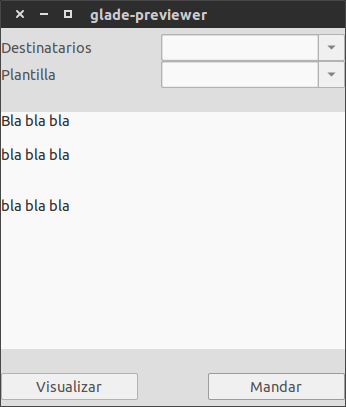
\includegraphics[width=0.4\textwidth]{graphics/sketch_ui.png}
    \caption{Bosquejo de la propuesta de Manuel}
\end{figure}

El Lunes 2 de Junio del 2014, después de la entrega de los documentos preeliminares, el profesor Adrian nos recuerda que la cantidad de días contemplados en la planeación exceden los días que faltan de clases (el proyecto tiene que estar terminado para el 8 de julio) por lo que algunos ajustes deben tomar lugar.

\section{Entrega de documentos preeliminares}
\textbf{Del Viernes 30 de Mayo al Martes 3 de Junio del 2014.}

Se realizó un documento preeliminar sobre el proyecto en donde se describen los siguientes temas:

\begin{itemize}
\item Presentación del equipo y la compañía
\item Descripción informal del proyecto
\item Presupuestación
\item Ámbito y descomposición del software
\item Planificación
\item Análisis de riesgo
\end{itemize}

Este documento se le entregó al profesor Adrian el día Lunes 2 de Junio del 2014 y nos dió unas cuantas correcciones anotadas sobre el trabajo el día Martes 3 de Junio. Describiré las correcciones y se tomarán en cuenta para el desarrollo de proyecto.

\subsection{Cambios en la presentación del equipo y la compañía}
Escribir textualmente sobre la ubicación de la compañía, Licenciatura en Ciencias de la Computación del Departamento de Matemáticas de la Universidad de Sonora.

Sabrosoftware ha aprendido de sus errores en el previo trabajo y planea posicionarse como \textbf{la compañía de desarrollo de software mejor calificada} de todo LCC.

Cuando se coloca el logo de la compañía sería bueno indicar cuando se diseñó el logo, quién lo diseñó y el lema de la compañía. Una propuesta es \emph{``El poder de mi software hará mi grandeza''}.

En la descripción del equipo de trabajo, colocar intereses, metas, gustos sobre nosotros; algo que indique en qué nos sentimos cómodos trabajando.

Definir un organigrama del equipo de trabajo o alguna representación que relacione los roles entre sí.

\subsection{Cambios en la descripción del proyecto}
Para la corrección creo que sería conveniente poner esto como introducción al ámbito y descomposición del problema, el cual debería ir antes que la presupuestación.

\subsection{Cambios en la presupuestación}
En el primer párrafo: \emph{La presupuestación del proyecto se realizó de dos maneras, \textbf{por líneas de código (LDC) y puntos de función (PF), las cuales se describen a continuación:}}.

El profesor comentó que el listado de actividades que establecí para realizar la presupuestación por líneas de código debería de ir en el ámbito y descomposición del problema.

Si consideramos la cantidad de líneas de código y las líneas de código al mes por persona, el tiempo es insuficiente considerando que somos tres personas programando en el equipo. Tendré que recalcular este presupuesto después de realizar la revisión a la descomposición del problema. También me hizo falta decir en que tanto tiempo terminaríamos el primer prototipo (por lo tanto la presupuestación se realizará después de tener el diagrama de Gantt).

Al calcular los puntos de función, debemos describir mejor el procedimiento. Tengo un escrito al respecto, faltaría transcribirlo. Ya que se tenga el valor numérico de los puntos de función se recomienda revisar el \emph{Pressman} para tomar datos de PF o bien utilizar la técnica \emph{COCOMO}. Creo que optaré por tomar los valores del \emph{Pressman}, ya que no recuerdo la técnica \emph{COCOMO}. Faltó especificar el costo total y el tiempo total.

\subsection{Cambios en el ámbito y descomposición del software}
Aquí tengo que incluír la parte de la descripción del problema y realizar una separación de componentes como en el listado de la presupuestación por líneas de código.

Recordar que el \emph{ámbito} está asociado a \textbf{¿Qué voy a resolver?} y la \emph{descomposición} está asociada a \textbf{¿Cómo lo voy a resolver?}.

\subsection{Cambios a la planificación}
Debido al poco tiempo que queda para culminar el trabajo, es necesario realizar unos cuantos ajustes a la planeación. Se mantiene igual la lista de actividades, sin embargo se reducen los tiempos para terminarlas.

\begin{itemize}
\item \textbf{2.1 y 2.3:} para el 4 de Junio del 2014.
\item \textbf{2.2 y 2.4:} del 5 de Junio al 8 de Junio del 2014.
\item \textbf{2.5 y 2.6:} del 5 de Junio al 8 de Junio del 2014.
\item \textbf{2.7:} del 5 de Junio al 15 de Junio del 2014.
\item \textbf{3.1, 3.2 y 3.3:} del 16 de Junio al 20 de Junio del 2014.
\item \textbf{4.1, 4.2 y 4.3:} del 21 de Junio al 26 de Junio del 2014.
\item \textbf{5.1, 5.2:} del 5 de Junio al 23 de Junio del 2014.
\item \textbf{5.3:} del 24 de Junio al 27 de Junio del 2014.
\item \textbf{6.1 y 6.2:} para el 28 de Junio del 2014.
\end{itemize}

\subsection{Cambios al análisis de riesgo}
No se realizaron observaciones a esta sección, no porque estuviera bien lo que se describe, si no porque el profesor no tuvo oportunidad de revisarlo. Mañana (Jueves 5 de Junio del 2014) le regresaré el trabajo para que revise esta última parte.

\section{Tiempo muerto}
\textbf{Viernes 6 de Junio del 2014}

No he podido invertirle mucho tiempo al desarrollo del proyecto. Este fin de semana no podré trabajar en el sistema, por lo que decidí comenzar a delegar trabajo a mis compañeros.

Para este fin de semana tengo planeado terminar las siguientes actividades:

\begin{itemize}
\item[2.1.] Determinar que necesitamos aprender.
\item[2.3.] ¿Cómo va a interaccionar el usuario con el sistema?
\item[2.2.] Establecer la interacción entre los diferentes componentes.
\item[2.4.] Diseñar la interfaz de usuario.
\item[2.5.] Elegir o diseñar los algoritmos para darle formato al oficio.
\item[2.6.] Elegir o diseñar los algoritmos para generar archivos PDF.
\end{itemize}

Las actividades 2.1 y 2.3 debieron de quedar terminadas para el 4 de Junio, entonces estas son prioridad, Daniel Contreras Mejía se encargará de concluirlas. Las actividades 2.2 y 2.4 debieron de ser iniciadas el 5 de Junio y tenemos para el Domingo 8 de Junio para terminarlas según el calendario definido, Daniel tiene asignadas estas actividades también.

Las actividades 2.5 y 2.6 le pertenecen a Francisco Manuel Valle Ruiz y debieron de ser comenzadas el 4 de Junio. Se tiene para el 8 de Junio para que se concluyan y no seguir atrasados.

Desafortunadamente aún no se comienza la implementación del programa, por lo que en la actividad 2.7 estamos retrasados también, pero esta la iniciaremos después de este fin de semana.

Hoy terminé de corregir el documento con las observaciones del profesor, tengo pendiente redactar la información de la entrevista con el profesor.

\end{document}
